\chapter[Revisão Estruturada da Literatura]{Revisão Estruturada da Literatura}

Neste capítulo será apresentado o estudo da Revisão Estruturada da Literatura, a fim de levantar o embasamento bibliográfico, respondendo à pergunta principal de pesquisa por intermédio das perguntas secundárias deste estudo.

\section{Protocolo}

O presente protocolo foi baseado no modelo proposto por \citeonline{kitchenham2007guidelines}. Dessa forma, será dividida em: planejamento, condução e síntese dos dados.

\subsection{\textit{String} de Busca}


As bases de dados acadêmicas indexam uma grande quantidade e diversidade de artigos, de diferentes áreas de conhecimento.  Dessa forma, para garantir a reprodutibilidade da pesquisa, requer o uso de um protocolo sistemático para a recuperação adequada daqueles artigos de maior interesse para a pesquisa. Tendo em vista o grau de sensibilidade da \textit{string} de busca, qualquer incoerência pode acarretar em um número excessivo de artigos sem relação com o tema da pesquisa, ou o inverso, ocorrer de ter um número insuficiente de estudos para responder à questão de pesquisa.

Por esta razão, o protocolo PICO foi utilizado para guiar a elaboração de uma \textit{string} de busca adequada às necessidades desta monografia. Como o protocolo tem origem na área de pesquisa da medicina, foi necessária uma adequação para sua aplicação na área de Engenharia de Software. Uma representação visual que facilita a compreensão do protocolo pode ser vista na Figura \ref{pico-adaptado}.

\begin{figure}[!h]
	\caption{Protocolo PICO}
	\centering
	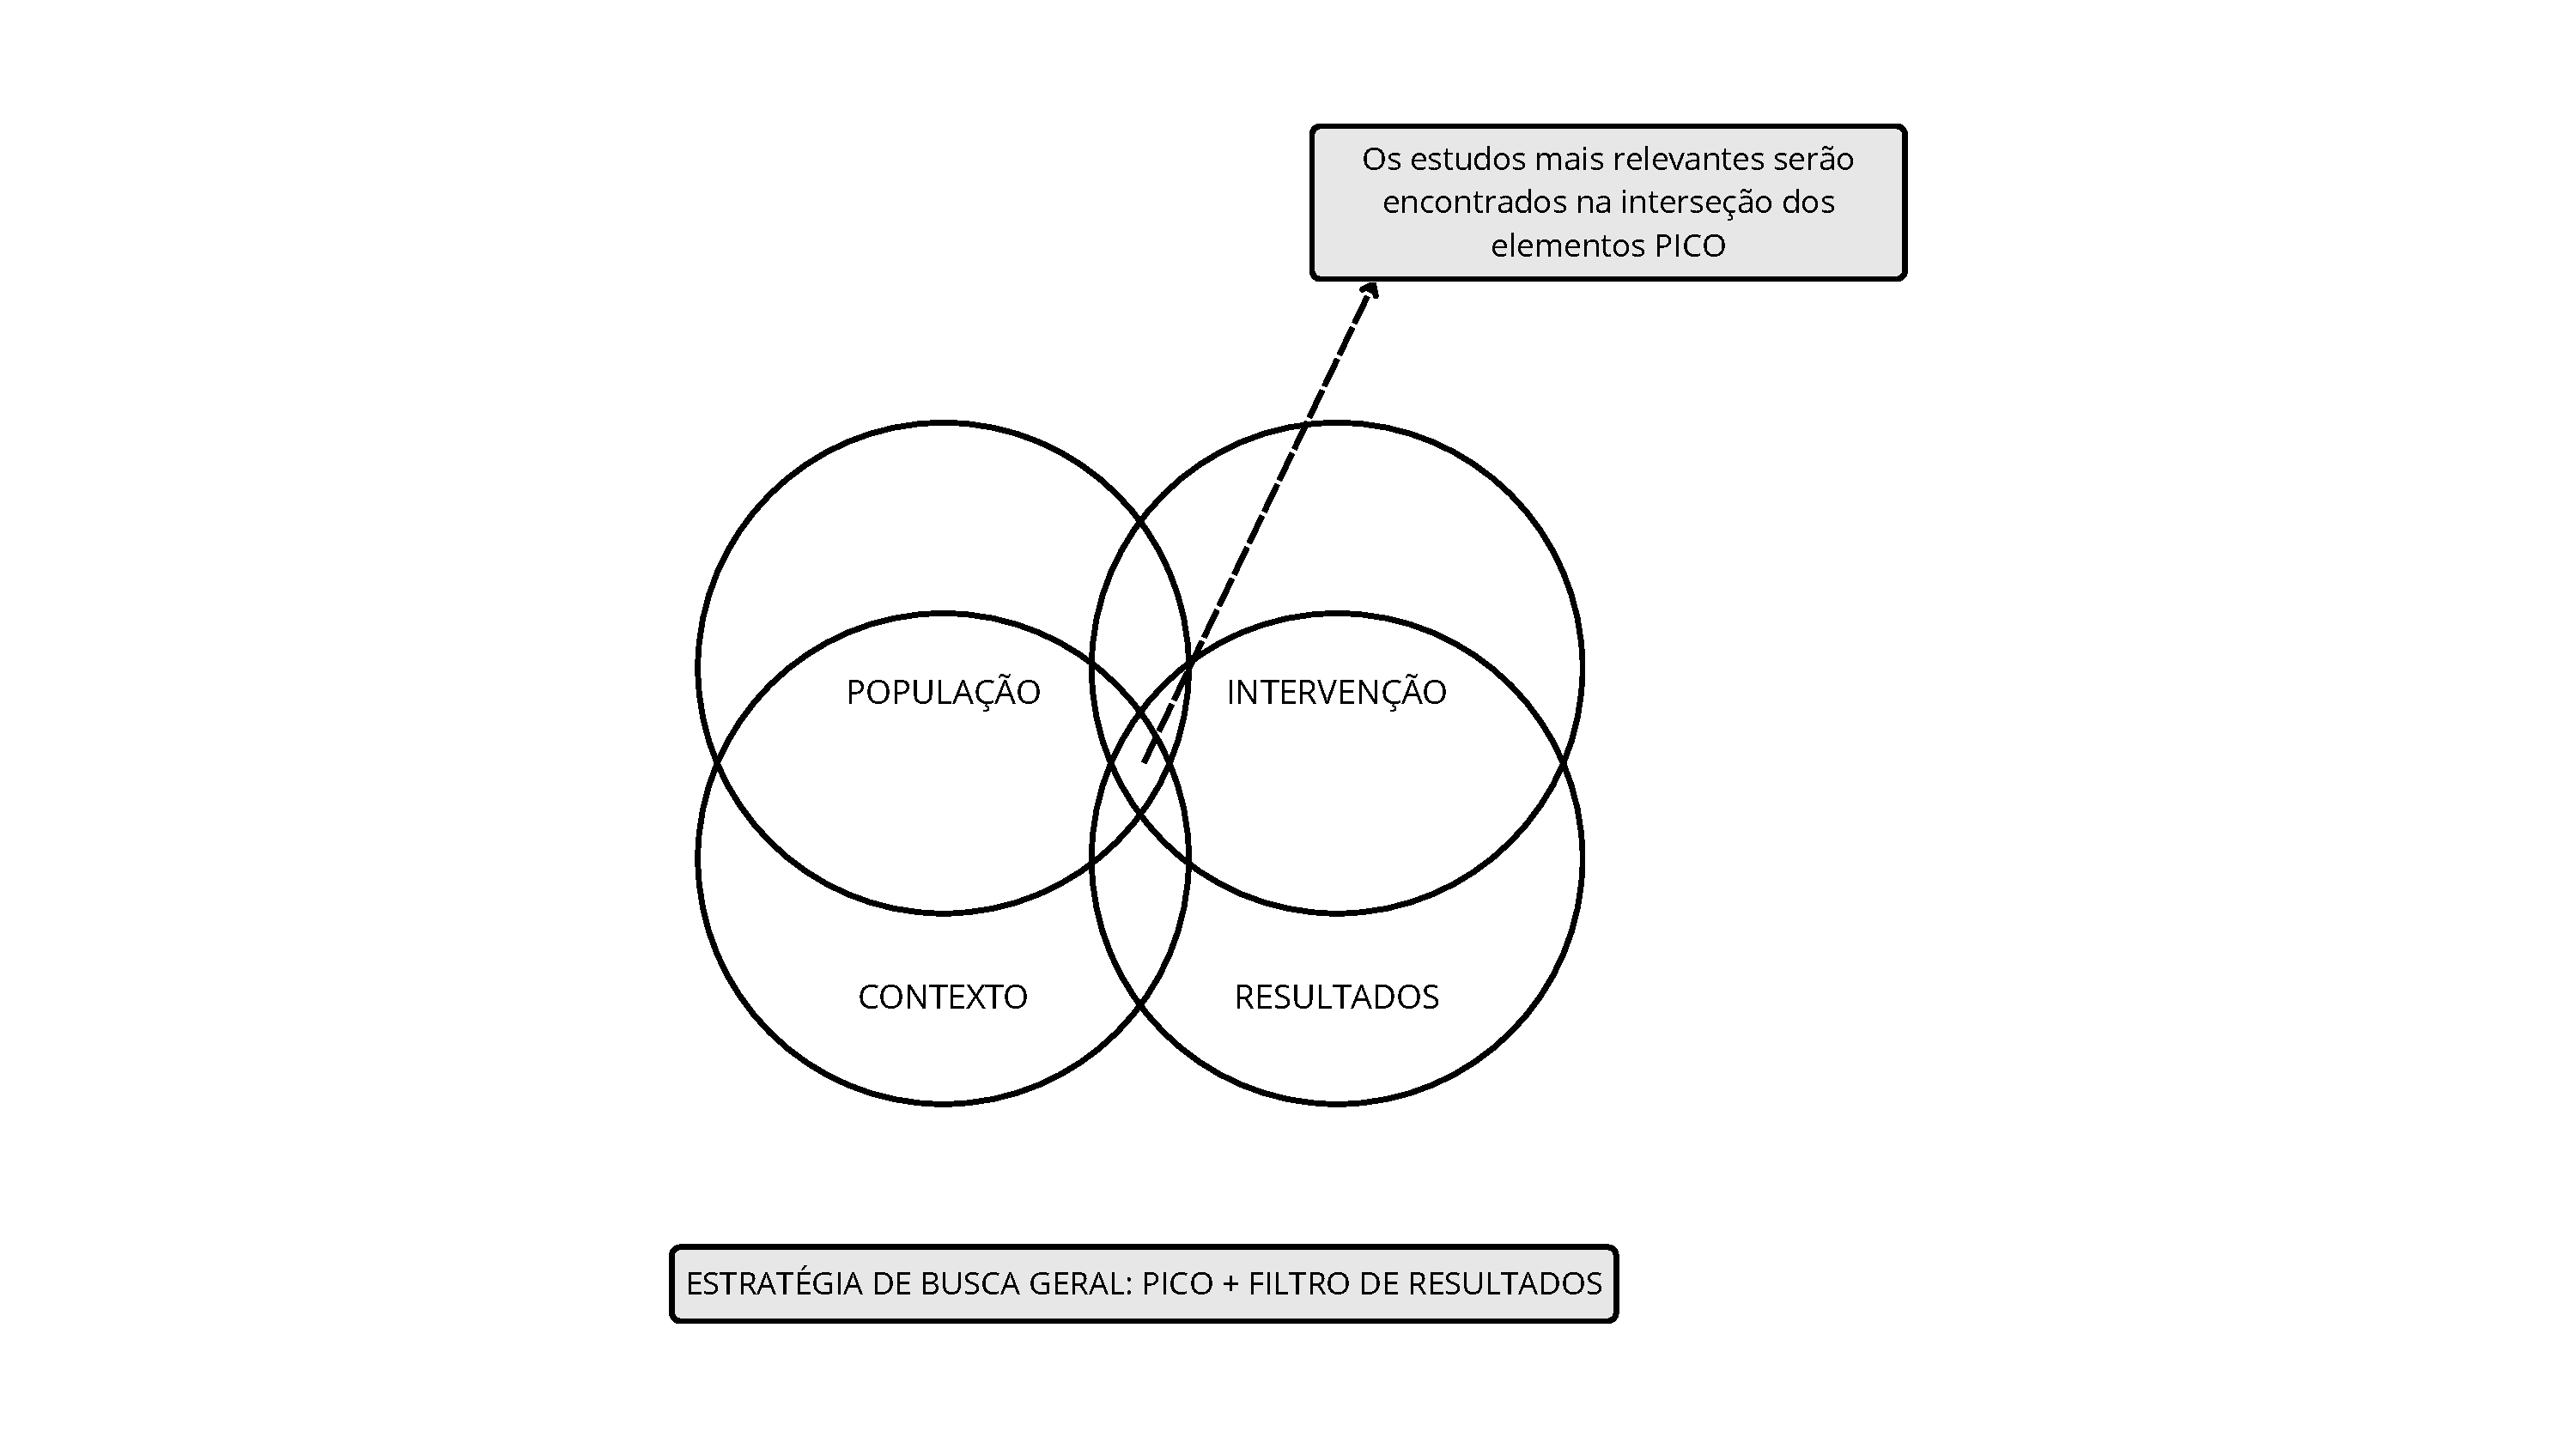
\includegraphics[width=1.5\textwidth]{figuras/pico-adaptado.pdf}
	{\small\textit{Fonte: Adaptado de \citeonline{pai2004systematic}.}}
	\label{pico-adaptado}
\end{figure}

As adaptações do protocolo, trouxeram novos significados aos elementos comumente utilizados. Por exemplo, o termo \textbf{Paciente}, utilizado para indicar o perfil do paciente, passa a representar a área de aplicação, ou a População, neste caso, a qualidade de software. A \textbf{Intervenção}, deixa de significar "tratamento médico" para se referir a metodologia, métodos, técnicas ou procedimentos avaliados para a medição de qualidade de software. Já ao que se trata de \textbf{Resultados} o significado se mantém, que no contexto dessa pesquisa refere-se aos efeitos ou consequências observadas; em especial foi adicionado um novo elemento relacionando o \textbf{Contexto}, que direcionou os resultados da pesquisa para o contexto de terceirização. Por fim, a \textbf{Comparação} que está relacionada a investigar como a intervenção proposta se relaciona com outras propostas de intervenção, essa não pode ser avaliada, visto que esta muito alinhada com os objetivos da medicina que na Engenharia de Software. A seguir, a definição de cada elementos usado no modelo estão definidos na Tabela~\ref{tab-PICO}


\begin{longtable}{|p{2.5cm}|p{3.5cm}|p{8.6cm}|}
    \caption{PICO Adaptado}
    \label{tab-PICO} \\
    \hline
    \textbf{Elementos} & \textbf{Termo Central} & \textbf{Termos Relacionados} \\
    \hline
    \endfirsthead

    \multicolumn{3}{l}{\small\textit{Continuação da Tabela~\ref{tab-PICO}}} \\
    \hline
    \textbf{Elementos} & \textbf{Termo Central} & \textbf{Termos Relacionados} \\
    \hline
    \endhead

    \hline
    \multicolumn{3}{r}{\small\textit{Continua na próxima página}} \\
    \endfoot

    \hline
    \endlastfoot

    \textbf{População} & Qualidade de Produto de Software & software product quality, Internal software product quality, Quality software, software product, Application Quality, Structural Quality, software development, systems development, code quality, Software health, structural health, product quality attribute*, quality-driven development, software characteristics, software artifact quality, codebase health, system quality, source code quality, software integrity, software robustness, software reliability \\
    \hline
    \textbf{Intervenção} & Medição de qualidade de Software & Maintainability, testability, modularity, quality model, software metric*, quality measure, measurement interpretation, release acceptance, release sign-off, ISO/IEC 25010, ISO 25010, ISO/IEC 9126, ISO 9126, ISO/IEC 25000, SQuaRE, QATCH, SQALE, Q-Rapids, technical debt, SQM, Software Quality Management, quality attributes, software measurement, code metrics, quality characteristics, internal metrics, structural metrics, complexity metrics, size metrics, quality indicators, software analytics, reusability, analyzability, modifiability, McCabe metric*, quality criteria, software evaluation, metric model \\
    \hline
    \textbf{Resultado e Contexto} & Terceirização & Outsourcing, External Development, Subcontracting, Third-party Development, Staff Augmentation, Dedicated Team, Dedicated Development Center, Project-based Outsourcing, IT Sourcing, offshoring, vendor*, supplier, public procurement, IT procurement, IS procurement, tendering, buyer-provider relations, contract management, backsourcing, insourcing, Brazil, Brazilian, Brasil, Lei 14.133, Lei 14133, Lei 8.666, Lei 8666, Lei 13.303, Lei 10.520, IN 01/2019, IN 94/2022, Instrução Normativa, Public Administration, Governmental, TCU, Tribunal de Contas, SLA, Service Level Agreement, Software acquisition, Information Technology Contracting, Public sector, GovTech, Bidding, Terms of Reference, vendor management, supplier selection, government contracting, public bidding, public purchasing, Request for Proposal, RFP, government procurement, e-procurement, software acquisition process, contract execution, software factory, fábrica de software, IT outsourcing, ITO, public contract*, government tender*, public administration IT, state-owned enterprise*, SISP, CGU, audit court*, contractual compliance, IT governance, governança de TI, Portaria 750, Portaria 750/2023, Portaria SGD, Portaria SGD/MGI, Secretaria de Governo Digital, Government Ordinance, Portaria \\
\end{longtable}

Para construir a estratégia de busca, utilizou-se o operador booleano \textit{OR} entre os termos de um mesmo elemento, visando maximizar a abrangência da pesquisa. Os grupos de termos foram combinados com o operador \textit{AND}, que foi aplicado para realizar a intersecção entre os diferentes componentes do protocolo PICO, garantindo a recuperação exclusiva de estudos alinhados às questões de pesquisa. Por fim, a sintaxe foi adaptada com os parâmetros específicos da base de dados SCOPUS, originando a seguinte expressão de busca:

\noindent\textit{TITLE-ABS-KEY ( ( "software product quality" OR "Internal software product quality" OR "Quality software" OR "software product" OR "Application Quality" OR "Structural Quality" OR "software development" OR "systems development" OR "code quality" OR "Software health" OR "structural health" OR "product quality attribute*" OR "quality-driven development" OR "software characteristics" OR "software artifact quality" OR "codebase health" OR "system quality" OR "source code quality" OR "software integrity" OR "software robustness" OR "software reliability" ) AND ( "Maintainability" OR "testability" OR "modularity" OR "quality model" OR "software metric*" OR "quality measure" OR "measurement interpretation" OR "release acceptance" OR "release sign-off" OR "ISO/IEC 25010" OR "ISO 25010" OR "ISO/IEC 9126" OR "ISO 9126" OR "ISO/IEC 25000" OR "SQuaRE" OR "QATCH" OR "SQALE" OR "Q-Rapids" OR "technical debt" OR "SQM" OR "Software Quality Management" OR "quality attributes" OR "software measurement" OR "code metrics" OR "quality characteristics" OR "internal metrics" OR "structural metrics" OR "complexity metrics" OR "size metrics" OR "quality indicators" OR "software analytics" OR "reusability" OR "analyzability" OR "modifiability" OR "McCabe metric*" OR "quality criteria" OR "software evaluation" OR "metric model" ) AND ( "Outsourcing" OR "External Development" OR "Subcontracting" OR "Third-party Development" OR "Staff Augmentation" OR "Dedicated Team" OR "Dedicated Development Center" OR "Project-based Outsourcing" OR "IT Sourcing" OR "offshoring" OR "vendor*" OR "supplier" OR "public procurement" OR "IT procurement" OR "IS procurement" OR "tendering" OR "buyer-provider relations" OR "contract management" OR "backsourcing" OR "insourcing" OR "Brazil" OR "Brazilian" OR "Brasil" OR "Lei 14.133" OR "Lei 14133" OR "Lei 8.666" OR "Lei 8666" OR "Lei 13.303" OR "Lei 10.520" OR "IN 01/2019" OR "IN 94/2022" OR "Instrução Normativa" OR "Public Administration" OR "Governmental" OR "TCU" OR "Tribunal de Contas" OR "SLA" OR "Service Level Agreement" OR "Software acquisition" OR "Information Technology Contracting" OR "Public sector" OR "GovTech" OR "Bidding" OR "Terms of Reference" OR "vendor management" OR "supplier selection" OR "government contracting" OR "public bidding" OR "public purchasing" OR "Request for Proposal" OR "RFP" OR "government procurement" OR "e-procurement" OR "software acquisition process" OR "contract execution" OR "software factory" OR "fábrica de software" OR "IT outsourcing" OR "ITO" OR "public contract*" OR "government tender*" OR "public administration IT" OR "state-owned enterprise*" OR "SISP" OR "CGU" OR "audit court*" OR "contractual compliance" OR "IT governance" OR "governança de TI" OR "Portaria 750" OR "Portaria 750/2023" OR "Portaria SGD" OR "Portaria SGD/MGI" OR "Secretaria de Governo Digital" OR "Government Ordinance" OR "Portaria" ) )}

\subsection{Seleção dos Artigos}


Com a \textit{string} de busca criada, foram definidos os critérios de inclusão e exclusão visando selecionar apenas os artigos mais pertinentes ao escopo da pesquisa. A partir da leitura do Título, Resumo e palavras-chaves dos artigos extraídos da \textit{string} de busca, foram rejeitados aqueles que não atendiam aos critérios de inclusão ou se enquadravam nos critérios de exclusão, e aceitados aqueles que atendiam a todos os critérios de inclusão. Posteriormente a partir do estudos selecionados foi preenchido o formulário de extração a fim de atender as perguntas de pesquisa secundárias. O Protocolo completo está definido na Tabela.

Ao todo foram analisados 501 artigos resultantes da string de busca, dos quais 50 foram selecionados e, destes, 30 foram lidos integralmente. Esses artigos foram obtidos na base de dados Scopus em 14 de maio de 2026. Os artigos selecionados estão dispostos na Tabela~\ref{tab-artigos-slr}.


A calibração da \textit{string} de busca consistia em verificar se o artigo \textit{Tools for monitoring software quality in information systems development and maintenance: five key challenges and a design proposal} de \citeonline{tools2020monitoring} estava presente na base de busca, o que confirmava que os resultados estavam dentro do escopo da pesquisa.


\begin{longtable}{|p{4.5cm}|p{10.6cm}|}
    \caption{Protocolo de Busca}
    \label{tab-protocolo} \\
    \hline
    \textbf{Item} & \textbf{Descrição} \\
    \hline
    \endfirsthead

    \multicolumn{2}{l}{\small\textit{Continuação da Tabela~\ref{tab-protocolo}}} \\
    \hline
    \textbf{Item} & \textbf{Descrição} \\
    \hline
    \endhead

    \hline
    \multicolumn{2}{r}{\small\textit{Continua na próxima página}} \\
    \endfoot

    \hline
    \endlastfoot

    Questões Secundárias de Pesquisa & \begin{enumerate}[nosep, leftmargin=*]
        \item Quais são os problemas identificados em qualidade do produto em produtos de softwares terceirizados?
        \item Quais são os modelos de qualidade para avaliação de manutenibilidade dos produtos de softwares utilizados na terceirização?
        \item Quais são as métricas utilizadas para aferição de modularidade e testabilidade em códigos?
        \item Quais ferramentas são utilizadas para coletas de dados para aferição de testabilidade e modularidade?
        \item Como os resultados das métricas e ferramentas de qualidade são agregados para embasar a avaliação e o aceite técnico da entrega de um fornecedor terceirizado?
        \item Quais são as práticas de desenvolvimento ou gerenciamento adotadas no processo de aferição da qualidade?
        \item Quais são as práticas adotadas no processo de aceitação de releases?
    \end{enumerate} \\
    \hline
    String de Busca & Tabela~\ref{tab-PICO} \\
    \hline
    Critérios de Inclusão & \begin{enumerate}[nosep, leftmargin=*]
        \item O artigo trata de qualidade interna de produto de software, ou de terceirização/contratação de desenvolvimento com abordagem de qualidade de produto
        \item O artigo propõe, avalia ou aplica modelos, métricas, indicadores ou ferramentas relacionados à Manutenibilidade ou suas subcaracterísticas
    \end{enumerate} \\
    \hline
    Critérios de Exclusão & \begin{enumerate}[nosep, leftmargin=*]
        \item O texto completo do artigo não está disponível
        \item O domínio de aplicação do estudo é exclusivamente não-web (ex: sistemas embarcados, sistemas de dispositivos móveis)
        \item Artigos duplicados
        \item O artigo não está escrito em Inglês ou português
        \item O artigo trata exclusivamente de qualidade de processo de desenvolvimento, governança de TI, gestão de contratos ou mercado de terceirização, sem avaliar qualidade interna do produto de software
    \end{enumerate} \\
    \hline
    Formulário de Extração & \begin{enumerate}[nosep, leftmargin=*]
        \item Título
        \item Resumo
        \item Ano de Publicação
        \item Fonte de Publicação
        \item Autores
        \item Palavras-chave
        \item Problemas identificados em qualidade do produto em produtos de softwares terceirizados
        \item Modelos de qualidade para avaliação de manutenibilidade na terceirização
        \item Métricas utilizadas para aferição de modularidade e testabilidade
        \item Análise de Modelo de Manutenibilidade
        \item Ferramentas utilizadas para coletas de dados
    \end{enumerate} \\
\end{longtable}

\begin{longtable}{|c|p{11.5cm}|c|}
    \caption{Artigos Selecionados da Revisão Estruturada da Literatura}
    \label{tab-artigos-slr} \\
    \hline
    \textbf{№} & \textbf{Título} & \textbf{Revista} \\
    \hline
    \endfirsthead

    \multicolumn{3}{l}{\small\textit{Continuação da Tabela~\ref{tab-artigos-slr}}} \\
    \hline
    \textbf{№} & \textbf{Título} & \textbf{Revista} \\
    \hline
    \endhead

    \hline
    \multicolumn{3}{r}{\small\textit{Continua na próxima página}} \\
    \endfoot

    \hline
    \endlastfoot

    1 & Empirical Investigation of Influencing Factors Regarding Offshore Outsourcing Decision of Application Maintenance~\cite{empirical2021offshore} & Sim \\
    \hline
    2 & Quality Management in Software Development~\cite{qualitymanagdev2024} & Sim \\
    \hline
    3 & Source Code Metrics: A Study on Scientific Publications in Brazilian Symposia and the Perception of Computing Students~\cite{sourcecode2024} & Sim \\
    \hline
    4 & Technical Debt Management in the Brazilian Federal Administration~\cite{souza2015technical} & Não \\
    \hline
    5 & Assessing technical debt in automated tests with codescene~\cite{tornhill2018codescene} & Não \\
    \hline
    6 & Alignment of Software Product Quality Goals in Two Outsourcing Relationships~\cite{alignment2026outsourcing} & Não \\
    \hline
    7 & A dynamic model of offshore software development~\cite{dynamic2001offshore} & Sim \\
    \hline
    8 & Metric based software project performance monitoring model~\cite{doraisamy2016metric} & Sim \\
    \hline
    9 & Effective quality management: Value- and risk-based software quality management~\cite{felderer2014eqm} & Sim \\
    \hline
    10 & An Importance-Performance Analysis Concerning the Quality of Indonesia's e-Procurement System Based on ISO/EIC 25010:2011~\cite{karsanti2023importance} & Não \\
    \hline
    11 & Importance of reuse and modularity in system architecture~\cite{dano2019modularity} & Não \\
    \hline
    12 & Understanding Technical Debt at the Code Level from the Perspective of Software Developers~\cite{sbes2017technical} & Não \\
    \hline
    13 & An empirical study on the importance of quality among offshore outsourced software development firms in Sri Lanka~\cite{csed2013quality} & Não \\
    \hline
    14 & Quality determinants in offshored IS projects: A comparison between projects completed within-budget and over-budget~\cite{qualitydeterminants} & Sim \\
    \hline
    15 & A Systematic Snapshot of Software Outsourcing Challenges~\cite{jebreen2023systematic} & Não \\
    \hline
    16 & Manual Tests Do Smell! Cataloging and Identifying Natural Language Test Smells~\cite{soares2023manual} & Não \\
    \hline
    17 & An Integrated Approach for Criteria Evaluation and Software Maintenance Process Management: Insights from Global Software Development Perspective~\cite{integrated2024maintenance} & Sim \\
    \hline
    18 & Using performance ethnography to explore the human aspects of software quality~\cite{performance2008ethnography} & Sim \\
    \hline
    19 & Evaluation of Determinants of Software Quality in Offshored Software Projects: Empirical Evidences From India~\cite{prabu2020offshore} & Sim \\
    \hline
    20 & A case of information systems pre-implementation failure: Pitfalls of overlooking the key stakeholders' interests~\cite{case2006failure} & Não \\
    \hline
    21 & An evaluation on software traceability in the context of MPS.BR; [Uma avaliação sobre rastreabilidade de software no contexto do MPS.BR]~\cite{mpsbr2021traceability} & Não \\
    \hline
    22 & Evaluating Software Quality: Application of ISO/IEC 25000 in Public and Private Sectors~\cite{iso25000public} & Sim \\
    \hline
    23 & The relationships between software development processes and software product quality~\cite{processes2013quality} & Sim \\
    \hline
    24 & Incorporating qualitative and quantitative factors for software defect prediction~\cite{defect2012prediction} & Sim \\
    \hline
    25 & CBR insight: Measure and visualize source code quality~\cite{cbr2019insight} & Sim \\
    \hline
    26 & Significant requirements engineering practices for software development outsourcing~\cite{iqbal2013requirements} & Não \\
    \hline
    27 & When management gets serious about managing software~\cite{jansma2005management} & Não \\
    \hline
    28 & Evaluation of expected software quality: A customer's viewpoint~\cite{gorski2006evaluation} & Sim \\
    \hline
    29 & Employability Assessment of Agile Methods for Software Quality: An Empirical Case Study~\cite{agile2022employability} & Não \\
    \hline
    30 & Measuring software product quality using ISO 9126: A systematic review~\cite{iso9126review} & Sim \\
    \hline
    31 & Managing technical debt: An industrial case study~\cite{managingtd2015} & Sim \\
    \hline
    32 & Evaluating software component quality from vendors using the primitive cognitive network process with ISO/IEC 9126~\cite{pcnp2019vendors} & Não \\
    \hline
    33 & Technical debt management in Brazilian software organizations: A need, an expectation, or a fact?~\cite{silva2018} & Sim \\
    \hline
    34 & Tools for monitoring software quality in information systems development and maintenance: five key challenges and a design proposal~\cite{tools2020monitoring} & Sim \\
    \hline
    35 & Quality of protection: Measuring the unmeasurable?~\cite{measuringunmeasurable} & Sim \\
    \hline
    36 & Study of a customer satisfaction-oriented model for outsourcing software quality management using Quality Function Deployment (QFD)~\cite{qfd2008outsourcing} & Não \\
    \hline
    37 & Individualizing Software Production: Bringing Work Back in Microsourcing Practices~\cite{microsourcing2020} & Sim \\
    \hline
    38 & Empirical analysis of intellectual property risks in software outsourcing~\cite{iprisk2020} & Não \\
    \hline
    39 & Investigating the effects of agile practices and processes on technical Debt-The viewpoint of the brazilian software industry~\cite{agile2018debt} & Não \\
    \hline
    40 & Promises of open source software for Australian government agencies - An exploratory study~\cite{opensource2015australia} & Não \\
    \hline
    41 & A consideration of the impact of interactions with module effects on the direct measurement of subjective software attributes~\cite{module2001subjective} & Sim \\
    \hline
    42 & Applying testing to enhance software product quality~\cite{applying2013testing} & Não \\
    \hline
    43 & Determinants of software quality in offshore development - An empirical study of an Indian vendor~\cite{gopal2011offshore} & Sim \\
    \hline
    44 & Software outsourcing quality achieved by global virtual collaboration~\cite{virtualcollab2006} & Sim \\
    \hline
    45 & An analysis of the factors determining software product quality: A comparative study~\cite{curcio2016} & Sim \\
    \hline
    46 & Characteristics of unmaintainable source code in software development by multiple organizations~\cite{unmaintainable2018} & Não \\
    \hline
    47 & ISO/IEC 9126: an experiment of application on Brazilian software products~\cite{iso91261999brazil} & Não \\
    \hline
    48 & Software quality and CASE tools~\cite{casetools1993} & Sim \\
    \hline
    49 & ISO9000-3 and software measurement~\cite{iso90003measurement} & Sim \\
    \hline
    50 & SOFTWARE QUALITY MEASUREMENT TOOLS AND TECHNIQUES~\cite{swebok1986tools} & Não \\
\end{longtable}


\begin{figure}[H]
	\centering
    \caption{Seleção dos Estudos}
	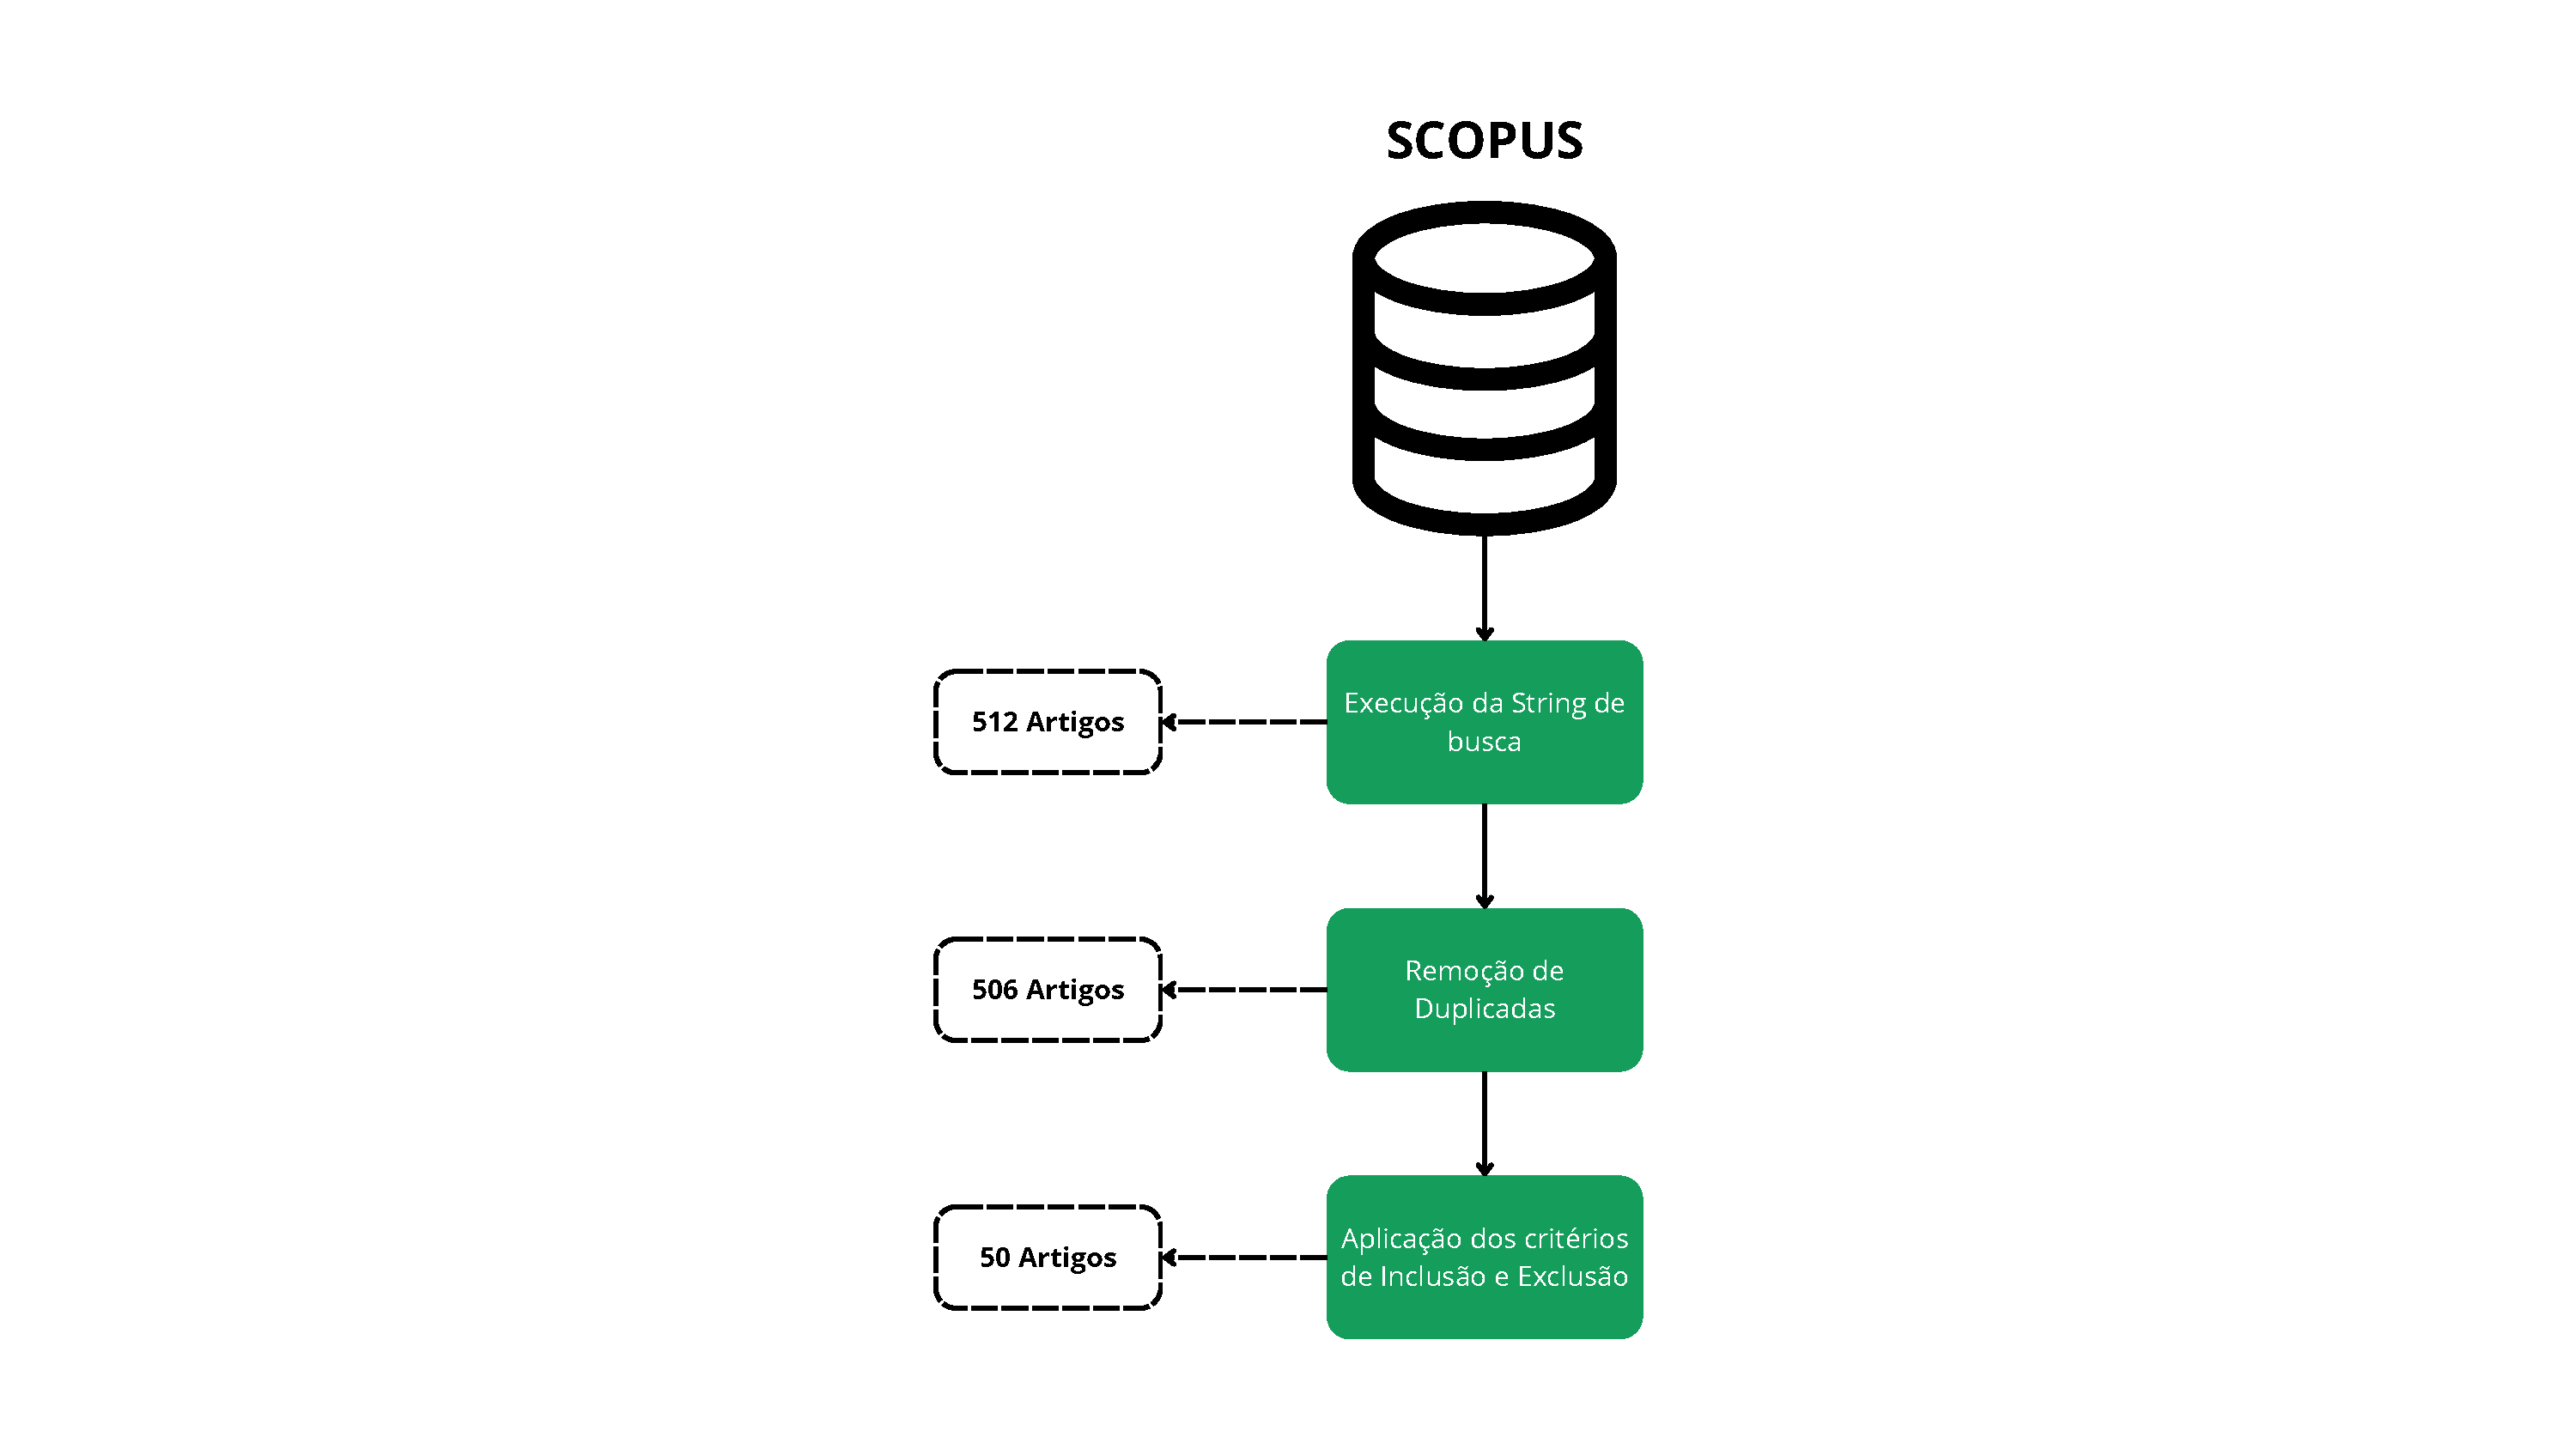
\includegraphics[width=1\textwidth]{figuras/selecao-estudos-rls.pdf}
    {\small\textit{Fonte: Autor.}}
	\label{selecao-estudos}
\end{figure}


\subsection{Resultados}

A condução da Revisão Estruturada foi dirigida pela ferramenta \textit{parsif.al}\footnote{Disponível em: \url{https://parsif.al/sousacmz/slr-1/}. Acesso em: 10 jul. 2026.}, e todos os dados extraídos a partir das leituras podem ser acessados por meio do repositório do \textit{Google Drive}\footnote{Disponível em: \url{https://docs.google.com/spreadsheets/d/1mSoV8ot8DjdiqXZrmOpguvC0lC5rHoZ6/edit?usp=drive_link&ouid=105819389515065669376&rtpof=true&sd=true}. Acesso em: 10 jul. 2026.}.

A análise dos 30 artigos lidos em toda a sua completude permitiu construir respostas para as sete questões secundárias de pesquisa. As sínteses são apresentadas nas subseções a seguir, organizadas de acordo com a sequência lógica de investigação: do reconhecimento dos problemas à caracterização das práticas de aceite.

\subsubsection{Problemas Identificados em Qualidade Interna de Produtos de Software Terceirizados}

A literatura evidencia que a falta de qualidade interna em produtos de software terceirizados constitui um problema estrutural e recorrente. \citeonline{jebreen2023systematic} identificaram, em um mapeamento sistemático de desafios globais em contratos de terceirização de TI, que a ausência de qualidade na entrega do produto figura como o segundo maior desafio relatado, afetando 33\% dos casos estudados.

Um dos fatores que explica esse cenário é a assimetria de perspectiva entre contratante e contratado. \citeonline{alignment2026outsourcing} demonstraram que desenvolvedores terceirizados, ao serem excluídos do planejamento estratégico da organização contratante, tendem a supervalorizar atributos de qualidade facilmente mensuráveis, como testabilidade e estatísticas de desempenho, por representarem evidências tangíveis do trabalho realizado, ao passo que subvalorizam atributos de manutenibilidade a longo prazo, cujas consequências não recaem sobre eles. Esse desalinhamento de incentivos conduz sistematicamente à degradação da qualidade estrutural do produto entregue.

No plano técnico, \citeonline{gopal2011offshore} apontaram que a incerteza de requisitos é o principal fator de risco em projetos de terceirização do desenvolvimento de software, impactando negativamente todos os atributos de qualidade, especialmente a manutenibilidade. A cada mudança de requisito não planejada são introduzidos defeitos estruturais que comprometem a modularidade e a coesão do código. Complementarmente, \citeonline{unmaintainable2018} demonstraram empiricamente que a substituição do fornecedor produz um efeito de deterioração arquitetural progressivo: arquivos com alto acoplamento tendem a concentrar os defeitos e a aumentar sua complexidade a cada ciclo de desenvolvimento conduzido por equipes distintas.

No contexto brasileiro, \citeonline{silva2018} identificaram que as organizações de software possuem baixo nível de maturidade na gestão da qualidade interna do produto e que os profissionais frequentemente possuem percepções equivocadas sobre o que constitui dívida técnica. Agrava esse quadro o fato de que, conforme apontado por \citeonline{tools2020monitoring}, as ferramentas de análise estática disponíveis produzem resultados incomparáveis entre si (uma mesma aplicação pode receber avaliações diametralmente opostas dependendo da ferramenta utilizada) e que um fornecedor pode deliberadamente selecionar a ferramenta mais permissiva ao seu conjunto de problemas no momento da entrega, inviabilizando o aceite técnico objetivo.

\subsubsection{Modelos de Qualidade para Avaliação de Manutenibilidade}

A revisão da literatura identificou um conjunto consolidado de modelos de qualidade de produto de software aplicáveis à avaliação de manutenibilidade, com diferentes graus de adoção e adequação ao contexto de terceirização.

O modelo prescrito pela norma ISO/IEC 9126 foi historicamente o mais adotado pela indústria. \citeonline{iso9126review} constataram que, dentre os estudos que utilizam modelos padronizados de qualidade de produto, a manutenibilidade é consistentemente a característica mais investigada. Contudo, os próprios autores observaram que 19,4\% dos estudos primários analisados apontam a genericidade do modelo como sua principal limitação prática, exigindo sempre algum grau de personalização para aplicação em domínios específicos. Essa constatação é relevante para o contexto contratual público, onde a ausência de parametrização prévia implica ambiguidade nas condições de aceite.

A norma ISO/IEC 25010, sucessora da ISO/IEC 9126, detalha a manutenibilidade em cinco subcaracterísticas (modularidade, reusabilidade, analisabilidade, modificabilidade e testabilidade), oferecendo uma decomposição mais granular e operacionalizável \cite{tools2020monitoring}. Essa estrutura tem sido adotada como referência nos estudos mais recentes, especialmente naqueles que propõem modelos de monitoramento contínuo da qualidade em contextos de desenvolvimento com múltiplos fornecedores.

O modelo SQALE (\textit{Software Quality Assessment based on Lifecycle Expectations}), implementado pela ferramenta SonarQube, representa uma abordagem distinta: ao invés de classificar os atributos de forma nominal, converte o débito técnico em uma estimativa financeira de esforço de correção \cite{letouzey2010}. Essa característica torna o SQALE particularmente adequado ao contexto de gestão contratual, uma vez que permite estabelecer limiares de aceitação expressos em horas de retrabalho — grandeza diretamente compreensível por gestores de contratos públicos. Sua utilização em contratos no âmbito da Administração Pública Federal brasileira foi documentada por \citeonline{souza2015technical}.

O \textit{framework} EQM (\textit{Effective Quality Management}), proposto por \citeonline{felderer2014eqm}, adapta o ciclo PDCA para o contexto de desenvolvimento terceirizado por meio de um ciclo IPDCA (Identificação, Planejamento, Execução, Verificação e Ação). O EQM organiza o processo de aferição de atributos de qualidade — incluindo a manutenibilidade — de forma integrada ao ciclo de entrega, atribuindo indicadores de produto (\textit{Product Quality Indicators — PQIs}) a cada fase do desenvolvimento.


\subsubsection{Métricas Utilizadas para Aferição de Modularidade e Testabilidade}

A literatura aponta métricas distintas para as duas subcaracterísticas investigadas. Para a modularidade, as métricas mais recorrentes referem-se ao acoplamento estrutural entre componentes. \citeonline{unmaintainable2018} adotaram as métricas de visibilidade \textit{fan-in} (VFI) e \textit{fan-out} (VFO) para classificar os arquivos de um sistema em quatro níveis de complexidade arquitetural (periférico, utilitário, controle e núcleo), demonstrando que arquivos de nível núcleo concentram as maiores taxas de defeitos. \citeonline{cbr2019insight} utilizaram as métricas CBO (\textit{Coupling Between Objects}), WMC (\textit{Weighted Methods per Class}) e RFC (\textit{Response For a Class}), propondo que um arquivo seja classificado como excessivamente complexo quando excede os limiares de ao menos quatro dessas métricas simultaneamente. A proporção de clones de código, presente em ambos os estudos, figura como indicador direto de baixa modularidade.

Para a testabilidade, a cobertura de código se destaca como a métrica mais diretamente aplicável. \citeonline{qualitymanagdev2024} propõem um modelo no qual a cobertura mínima de testes unitários é fixada em 80\%, com exigência de 100\% de cobertura nos testes de integração como condição para a aceitação de um incremento de software. A complexidade ciclomática de McCabe, calculada a partir do número de caminhos independentes de execução em um módulo, é apontada por \citeonline{tornhill2018codescene} como o principal preditor de dificuldade de teste: módulos com alta complexidade ciclomática exigem um número proporcionalmente maior de casos de teste para cobertura adequada, tornando-se candidatos prioritários à refatoração antes do aceite. \citeonline{applying2013testing} propuseram a métrica EFD (\textit{Effectiveness in Fault Detection}), calculada como a razão entre falhas encontradas pela equipe de testes e o total de falhas identificadas em produção, como indicador objetivo da eficácia do processo de teste aplicado ao produto entregue.

É importante destacar que \citeonline{sourcecode2024} identificaram, em um mapeamento sistemático do contexto brasileiro, uma lacuna entre a produção acadêmica de métricas de código e seu uso efetivo na indústria: as métricas propostas são em grande parte descritivas, sem associação clara a critérios operacionais de qualidade. Esse achado é convergente com a constatação de \citeonline{measuringunmeasurable} de que as métricas de software não possuem, isoladamente, capacidade preditiva ou de controle confiável sobre a qualidade global de um sistema, reforçando a necessidade de uso combinado de múltiplas métricas integradas em um modelo de referência.

\subsubsection{Ferramentas Utilizadas para Coleta de Dados}

\citeonline{tools2020monitoring} conduziram o estudo de maior abrangência sobre ferramentas de análise estática aplicáveis ao monitoramento de qualidade de software em contextos de desenvolvimento e manutenção, comparando seis plataformas amplamente utilizadas: SonarQube\footnote{Disponível em: \url{https://www.sonarqube.org}. Acesso em: 10 jul. 2026.}, Better Code Hub\footnote{Disponível em: \url{https://bettercodehub.com}. Acesso em: 10 jul. 2026.}, CAST Highlight\footnote{Disponível em: \url{https://www.castsoftware.com/highlight}. Acesso em: 10 jul. 2026.}, Codacy\footnote{Disponível em: \url{https://www.codacy.com}. Acesso em: 10 jul. 2026.}, Codebeat\footnote{Disponível em: \url{https://codebeat.co}. Acesso em: 10 jul. 2026.} e Code Climate Quality\footnote{Disponível em: \url{https://codeclimate.com/quality}. Acesso em: 10 jul. 2026.}. O SonarQube destacou-se como a ferramenta mais adequada ao contexto de gestão contratual, por combinar extração automática de métricas com o modelo SQALE de rastreabilidade e por disponibilizar painéis de conformidade auditáveis por terceiros. Contudo, os autores alertam para limitações críticas comuns a todas as ferramentas analisadas: foco exclusivo no código-fonte, ignorando configurações e comportamento em tempo de execução; incapacidade de avaliar a arquitetura entre componentes escritos em linguagens distintas; e inconsistência dos limiares adotados, que são frequentemente proprietários e variam entre ferramentas de forma não documentada.

O SonarQube aparece ainda como ferramenta de referência em \citeonline{silva2018} para coleta de métricas de dívida técnica, e é indicado por \citeonline{iso25000public} especificamente como suporte à avaliação de manutenibilidade segundo a ISO/IEC 25000. Para análise de testabilidade e dívida técnica em suítes de testes automatizados, \citeonline{tornhill2018codescene} propuseram o uso do CodeScene\footnote{Disponível em: \url{https://codescene.com}. Acesso em: 10 jul. 2026.}, ferramenta que combina análise de frequência de mudança por método com métricas de complexidade ciclomática para identificar componentes com maior risco de acúmulo de dívida técnica.

Para análise de dependências arquiteturais e clones de código — métricas centrais para a avaliação de modularidade —, \citeonline{unmaintainable2018} utilizaram o Understand\footnote{Disponível em: \url{https://www.scitools.com}. Acesso em: 10 jul. 2026.} (Scientific Toolworks) para extração de métricas de visibilidade VFI/VFO, combinado com Nicad Clone Detector\footnote{Disponível em: \url{https://www.txl.ca/txl-nicaddownload.html}. Acesso em: 10 jul. 2026.} para C\# e PMD-CPD\footnote{Disponível em: \url{https://pmd.github.io}. Acesso em: 10 jul. 2026.} para C++ e Java. \citeonline{applying2013testing} demonstraram o uso integrado de Mantis\footnote{Disponível em: \url{https://www.mantisbt.org}. Acesso em: 10 jul. 2026.}, TestLink\footnote{Disponível em: \url{https://testlink.org}. Acesso em: 10 jul. 2026.} e Subversion\footnote{Disponível em: \url{https://subversion.apache.org}. Acesso em: 10 jul. 2026.} para estabelecer rastreabilidade entre defeitos, casos de teste e versões do produto, fornecendo a base empírica para o cálculo da métrica EFD no processo de aceite.

\subsubsection{Agregação de Resultados para Embasar o Aceite Técnico}

A literatura apresenta diferentes abordagens para a agregação dos resultados das métricas e ferramentas em um processo formal de aceite técnico. O aspecto mais recorrente é a necessidade de que os critérios de aceite sejam definidos antecipadamente — preferencialmente no próprio instrumento contratual — e não no momento da entrega, quando o fornecedor já detém assimetria de informação sobre o estado real do produto \cite{tools2020monitoring}.

\citeonline{souza2015technical} apresentaram, no contexto da Administração Pública Federal brasileira, o processo SCRUM-GeDDAS, no qual o valor da dívida técnica acumulada no código entregue é calculado e monetizado por meio do modelo SQALE, servindo como critério quantitativo de aceite ou rejeição do \textit{release}. Esse modelo tem a vantagem de traduzir as métricas técnicas para uma linguagem financeira diretamente aplicável à gestão de contratos administrativos.

\citeonline{felderer2014eqm} propõem que o aceite seja precedido por um processo de transparência total das atividades de garantia de qualidade: todos os indicadores de produto e suas medidas de validação devem ser publicados e acordados entre contratante e contratado antes do início do desenvolvimento, de modo que a aprovação ou rejeição de uma entrega seja baseada em evidências previamente pactuadas. Quando os recursos orçamentários se esgotam antes da validação de todas as funcionalidades, os autores propõem a formalização explícita das funções não validadas — denominada lacuna de validação transparente —, com concordância de todos os \textit{stakeholders} para a aceitação parcial.

No contexto governamental, \citeonline{gorski2006evaluation} descreveram um processo de auditoria estruturado em seis dimensões: processos e métodos, produtos de análise, produtos de \textit{design}, implementação e código, testes e manuais de usuário, fundamentado em rastreabilidade formal entre requisitos legais, procedimentos de negócio e casos de teste. Nesse modelo, pontuações baixas em qualquer dimensão não geram rejeição automática, mas um relatório estruturado de riscos enviado ao fornecedor com recomendações de correção, conferindo ao processo de aceite um caráter iterativo e auditável. \citeonline{pcnp2019vendors} propuseram, por sua vez, a aplicação do método P-CNP (\textit{Primitive Cognitive Network Process}) integrado aos critérios da ISO/IEC 9126 para contornar os problemas de percepção cognitiva humana presentes nos métodos de tomada de decisão multicritério tradicionais, produzindo um escore global comparável entre fornecedores concorrentes de forma matematicamente fundada.

\subsubsection{Práticas de Desenvolvimento e Gerenciamento Adotadas no Processo de Aferição da Qualidade}

A literatura identifica um conjunto diversificado de práticas organizacionais e técnicas que suportam a aferição contínua da qualidade interna em contextos de terceirização. Nos estudos de maior aderência ao contexto público brasileiro, \citeonline{souza2015technical} descreveram o processo SCRUM-GeDDAS, que incorpora marcos formais de medição de dívida técnica entre os ciclos de entrega. A análise classificatória de arquivos por nível de acoplamento arquitetural, com foco de auditoria nos componentes de nível núcleo identificados pelos maiores valores de VFI, é recomendada por \citeonline{unmaintainable2018} como prática preventiva para reduzir o risco de regressão de qualidade em entregas sucessivas.

A \textit{Definition of Done} — conjunto de critérios técnicos mínimos para que uma unidade de código seja aceita na base do produto — é apontada por \citeonline{silva2018} como a prática de maior proeminência entre profissionais brasileiros, funcionando como um portão de qualidade que impede a acumulação de dívida técnica antes que ela alcance os estágios formais de entrega. No plano do processo de desenvolvimento, \citeonline{agile2018debt} identificaram que refatoração e iterações curtas são as práticas percebidas como mais eficazes para controlar a dívida técnica no contexto brasileiro, enquanto \citeonline{gopal2011offshore} e \citeonline{prabu2020offshore} destacam que a adoção de modelos de maturidade de processo — como o CMMI Nível 5 — e de mecanismos de transferência e integração de conhecimento entre equipes são determinantes para a manutenibilidade dos produtos entregues.

A co-criação do modelo de qualidade entre o gestor do contrato e um consultor especializado é proposta por \citeonline{tools2020monitoring} como alternativa à imposição unilateral de métricas pela ferramenta ou pelo fornecedor. Nesse modelo, as métricas relevantes ao contexto específico do projeto são selecionadas e parametrizadas em conjunto, e a forma de cálculo da nota final de qualidade é documentada de maneira rastreável e transparente. \citeonline{alignment2026outsourcing} propõem complementarmente a adoção da Theory-W (\textit{Win-Win}), que busca alinhar os objetivos de qualidade de contratante e contratado desde o início do contrato, reduzindo os desvios de incentivo que historicamente levam os fornecedores a subvalorizar atributos de manutenibilidade.

\subsubsection{Práticas Adotadas no Processo de Aceitação de Releases}

O processo formal de aceitação de \textit{releases} em contextos de desenvolvimento terceirizado emerge na literatura como uma etapa crítica para a garantia da qualidade interna do produto. \citeonline{qualitymanagdev2024} descrevem um modelo de \textit{pipeline} de aceite estruturado em estágios sequenciais: execução de testes automatizados, verificação de cobertura unitária com limiar mínimo de 80\%, confirmação de cobertura total nos testes de integração e verificação de vulnerabilidades e conformidade com padrões de código. Nesse modelo, cada transição entre os ambientes de desenvolvimento, teste e produção é condicionada à aprovação de todos os estágios anteriores.

A definição antecipada e contratual das métricas e ferramentas de aferição é o mecanismo de aceite mais enfatizado na literatura. \citeonline{tools2020monitoring} argumentam que a especificação prévia das ferramentas e limiares de qualidade no instrumento contratual é a única forma de garantir que o aceite técnico seja baseado em evidências objetivas e não manipuláveis pelo fornecedor, eliminando a assimetria de informação que ocorre quando essa escolha é feita no momento da entrega. Complementando essa perspectiva, \citeonline{unmaintainable2018} recomendam que o aceite de \textit{releases} em transições de fornecedor inclua obrigatoriamente uma etapa de refatoração preventiva dos arquivos com maior acoplamento, uma vez que aceitar código altamente acoplado cria uma dívida estrutural que se torna progressivamente mais cara de eliminar em ciclos futuros.

\citeonline{gorski2006evaluation} demonstraram, no contexto de um grande sistema governamental, que a rastreabilidade entre requisitos e casos de teste é condição necessária — mas não suficiente — para o aceite: é preciso ainda que o ambiente de teste utilizado pelo fornecedor seja consistente com o ambiente de produção do contratante. Esse requisito, frequentemente negligenciado em contratos de TI públicos, impacta diretamente a validade das métricas de cobertura e testabilidade coletadas. \citeonline{silva2018} reforçam essa perspectiva ao apontar a \textit{Definition of Done} como instrumento de aceitação preventiva: ao exigir que cada unidade de código cumpra os critérios técnicos antes de ser integrada à base, reduz-se o acúmulo de problemas de qualidade que seriam detectados apenas no momento do \textit{release} formal.

\subsubsection{Síntese dos Resultados}

O corpus analisado nesta revisão estruturada da literatura é composto por 50 artigos candidatos obtidos na base de dados Scopus (Figura \ref{artigos-ano}), dos quais 30 foram lidos integralmente, com extração de dados, por atenderem aos critérios de inclusão estabelecidos no protocolo. Dos 20 artigos restantes, 15 foram excluídos por tratarem exclusivamente de qualidade de processo sem avaliação da qualidade interna do produto, ou por terem como domínio de aplicação exclusivo sistemas embarcados ou dispositivos móveis. Já os outros 5, por indisponibilidade do texto completo.

Quanto à natureza dos veículos de publicação, o corpus total de 50 artigos candidatos é composto predominantemente por periódicos científicos, que representam 54\% das publicações, seguidos por artigos publicados em anais de conferências, com 34\% do total. Simpósios respondem por 6\% do corpus, enquanto \textit{workshop}, capítulo de livro e uma publicação sem veículo identificado correspondem a 2\% cada. Considerando apenas os 30 artigos lidos, a proporção de periódicos se mantém como maioria, com os anais de conferências como segundo grupo mais expressivo. Essa distribuição reflete o caráter consolidado do tema na literatura, com predominância de estudos submetidos a ciclos de revisão mais rigorosos e de maior durabilidade científica.

A distribuição temporal dos artigos incluídos abrange um intervalo de quatro décadas, com os primeiros estudos datando de 1986, época em que foram sistematizadas as métricas clássicas de software, como a complexidade ciclomática de McCabe e as métricas de Halstead \cite{swebok1986tools}, até 2026, demonstrando a continuidade e a atualidade do tema. A concentração de publicações se dá no período entre 2013 e 2024, com destaque para 2018, ano com o maior número de artigos incluídos no corpus. Essa tendência reflete o crescimento da produção científica sobre qualidade interna de produto no contexto de terceirização a partir da disseminação das metodologias ágeis e do avanço das ferramentas de análise estática automatizada.

\begin{figure}[H]
	\centering
    \caption{Artigos por ano}
	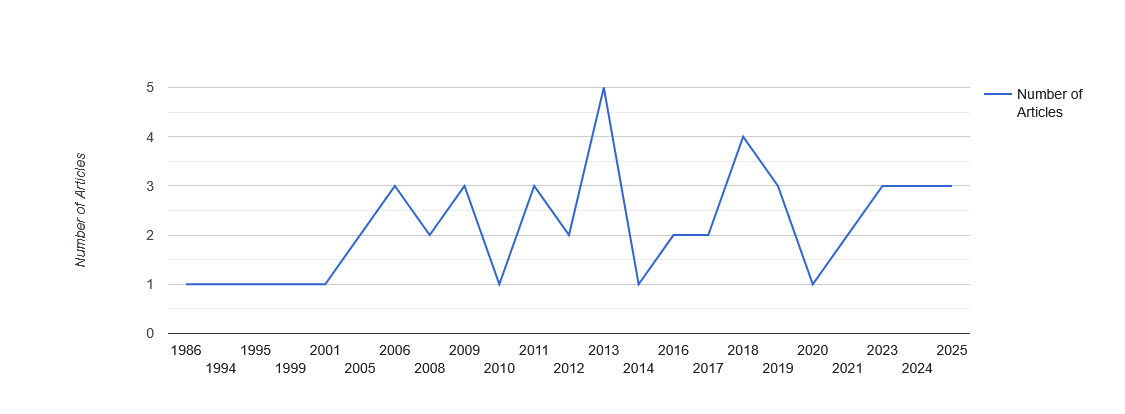
\includegraphics[width=1\textwidth]{figuras/artigos-ano.png}
    {\small\textit{Fonte: Parsif.al}}
	\label{artigos-ano}
\end{figure}


Do total de artigos lidos em toda a sua completude, 14 respondem diretamente à questão principal de pesquisa e 16 a respondem parcialmente, o que significa que a totalidade do corpus analítico contribui, em certa medida, para a caracterização da aceitação de versões de produtos de software terceirizados com base em critérios de manutenibilidade. A ausência, no conjunto de artigos analisados, de um modelo empiricamente validado que integre métricas concretas com limiares operacionais verificáveis para Modularidade e Testabilidade em um \textit{framework} formal de aceite contratual constitui a principal lacuna identificada e confirma a pertinência e a originalidade da presente pesquisa.

\section*{Declaração de Uso de Inteligência Artificial Generativa}
\addcontentsline{toc}{section}{Declaração de Uso de Inteligência Artificial Generativa}

Em atendimento à Portaria CNPq nº 2.664/2026, o autor declara o uso das seguintes ferramentas de Inteligência Artificial Generativa na elaboração deste capítulo:

\begin{enumerate}
    \item \textbf{Ferramenta:} Claude Sonnet 4.5 \\
    \textbf{Empresa desenvolvedora:} Anthropic \\
    \textbf{Versão/período de uso:} maio de 2026 \\
    \textbf{Finalidade:} geração da tabela de artigos selecionados e da síntese da distribuição temporal/geográfica dos artigos incluídos na revisão \\
    \textbf{Parte do trabalho aplicada:} Tabela~\ref{tab-artigos-slr} (Artigos Selecionados da Revisão Estruturada da Literatura) e subseção "Síntese dos Resultados"

    \item \textbf{Ferramenta:} Gemini 3.1 Pro \\
    \textbf{Empresa desenvolvedora:} Google \\
    \textbf{Versão/período de uso:} maio de 2026 \\
    \textbf{Finalidade:} geração da tabela de artigos selecionados e da síntese da distribuição temporal/geográfica dos artigos incluídos na revisão \\
    \textbf{Parte do trabalho aplicada:} Tabela~\ref{tab-artigos-slr} (Artigos Selecionados da Revisão Estruturada da Literatura) e subseção "Síntese dos Resultados"

    \item \textbf{Ferramenta:} Claude Sonnet 4.6 \\
    \textbf{Empresa desenvolvedora:} Anthropic \\
    \textbf{Versão/período de uso:} julho de 2026 \\
    \textbf{Finalidade:} revisão ortográfica, gramatical e semântica de rascunhos previamente elaborados pelo autor, sem alteração do conteúdo ou sentido do texto \\
    \textbf{Parte do trabalho aplicada:} Capítulo 3 integralmente
\end{enumerate}

O autor declara estar ciente do uso das ferramentas de Inteligência Artificial Generativa acima descritas e assume integral responsabilidade pelo conteúdo, pela veracidade das informações e pelas conclusões apresentadas neste capítulo, tendo revisado criticamente todo o material gerado ou auxiliado por tais ferramentas.